% documentclass
% set font size=11 (11pt)
% set paper format=A4 (a4paper)
% set equation alignment to left (fleqn)
\documentclass[11pt,a4paper,fleqn]{article}


% Preamble
% use the inputenc and fontenc packages to use French accents
\usepackage[utf8]{inputenc}
\usepackage[T1]{fontenc}
% for matrices / vectors
\usepackage{amsmath}
% allow for arbitrary font size
\usepackage{anyfontsize}
% for color
\usepackage{xcolor}
% for pseudocolor
\usepackage{algorithm,algpseudocode}
% for code samples
\usepackage{listings}
% set the font as Time New Roman (the Latex equivalent, at least)
% \usepackage{mathptmx}
% set the size of the document margins using the geometry package
\usepackage[lmargin=0.97in,rmargin=0.97in,tmargin=1.4in,bmargin=1.4in]{geometry}
% turn the color of footnote markers to black
\renewcommand\thefootnote{\textcolor{black}{\arabic{footnote}}}
% suppress indents on footnotes
\usepackage[hang,flushmargin]{footmisc}
% automatically generates colored brackets around references
\usepackage{fncylab} \labelformat{equation}{(#1)}
% supress indent on new paragraphs
\setlength{\parindent}{0pt}
% use the amsmath package to include mathematical symbols
\usepackage{amsmath}
% suppress the space between the left margin and the equations (fleqn still leaves some space by default)
\setlength{\mathindent}{0pt}
% create a new environment to left flush the equation with the align environment
\makeatletter
\newenvironment{lflalign}{ \vspace{-3mm}%
  \def\align@preamble{%
    &\strut@
    \setboxz@h{\@lign$\m@th\displaystyle{####}$}%
    \ifmeasuring@\savefieldlength@\fi
    \set@field
    \hfil
    \tabskip\z@skip
    &\setboxz@h{\@lign$\m@th\displaystyle{{}####}$}%
    \ifmeasuring@\savefieldlength@\fi
    \set@field
    \hfil
    \tabskip\alignsep@
  }
  \flalign}
{\endflalign}
\makeatother
% use the ammssymb package to use mathematical symbols
\usepackage{amssymb}
% create new commands for mathematical symbols
\DeclareMathOperator{\N}{\mathbb{N}}
\DeclareMathOperator{\Z}{\mathbb{Z}}
\DeclareMathOperator{\Q}{\mathbb{Q}}
\DeclareMathOperator{\R}{\mathbb{R}}
\DeclareMathOperator{\Pb}{\mathbb{P}}
% declare the cmsy (computer modern symbol) math alphabet to define appropriate fonts for the U and N mathematical symbols
\DeclareMathAlphabet\mathbcal{OMS}{cmsy}{m}{n}
% create new commands for mathematical symbols
\DeclareMathOperator{\E}{\mathbcal{E}}
\DeclareMathOperator{\Ex}{\mathbb{E}}
\DeclareMathOperator{\F}{\mathbcal{F}}
\DeclareMathOperator{\G}{\mathbcal{G}}
\DeclareMathOperator{\M}{\mathbcal{M}}
\DeclareMathOperator{\HH}{\mathbcal{H}}
\DeclareMathOperator{\QQ}{\mathbcal{Q}}
\DeclareMathOperator{\PP}{\mathbcal{P}}
\DeclareMathOperator{\Noo}{\mathbcal{N}}
\DeclareMathOperator{\U}{\mathbcal{U}}
% use the bbm package to be able to use the double stroke 1 for the indicator function
\usepackage{bbm}
\DeclareMathOperator{\ind}{\mathbbmss{1}}
% use the bm package to use bold characters in math mode
\usepackage{bm}
% create a new command for black square bullets
\newcommand{\bs}{\scalebox{0.7}{$\blacksquare$} \hspace{2mm}}
% use the relsize package to be abe to change the size of mathematical symbols
\usepackage{relsize}
% define a new command for in-line small summation
\newcommand{\ssumm}[2]{\underset{\scriptscriptstyle #1}{\overset{\scriptscriptstyle #2}{\mathlarger{\mathlarger{\mathlarger{\Sigma}}}}} \hspace{0.5mm}}
% define a new command for in-line small products
\newcommand{\sprod}[2]{\underset{\scriptscriptstyle #1}{\overset{\scriptscriptstyle #2}{\mathlarger{\mathlarger{\mathlarger{\Pi}}}}} \hspace{0.5mm}}
% Use the caption package to customize captions (titles) of tables and graphs
\usepackage[font=small,labelfont=bf]{caption}
% use float package to force figure the be positioned where indicated
\usepackage{float}
% use the graphicx package to be able to resize tables
\usepackage{graphicx}


\begin{document}

% command to check unused bibliography entries
% \nocite{*}
{\fontsize{12pt}{22pt} \textbf{Learning theory for classification}\par}

\vspace{5mm}

$g$ is the \textit{classifier}.

$$g: \mathcal{X} \to \mathcal{Y}$$
$$~~~~~~~~~~\mathbb{R}^d \to \{0,1\}$$

To model the learning problem, we use the pair $(X,Y)$ described by $(\mu, \eta)$ where $\mu$ is the probability measure:

$$\mu(A) = \mathbb{P}(X \in A)$$

And $\eta$ is the regression of $Y$ on $X$:

$$\eta(X) = \mathbb{P}(Y=1 | X=x) = \mathbb{E}[Y | X=x]$$

$\eta$ is also called the \textit{a posteriori probability}.

The Bayes classifier is:

  \begin{equation}
    \begin{cases}
      1 & \text{if}\ \eta(x) > 1/2 \\
      0 & \text{otherwise}
    \end{cases}
  \end{equation}

Or, if $\mathcal{Y}$ is $\{-1,1\}$, we write the classifier as such: $g(x) = 2 \mathbbm{1}\{ \eta(x)>1/2\}-1$.

\vspace{5mm}

\underline{Theorem}:

\vspace{5mm}

For any classifier g: $\mathbb{R}^d \to \{0,1\}$,
$$\mathbb{P}(g^*(X) \neq Y) \le \mathbb{P}(g(X) \neq Y)$$

In other words, the Bayes classifier is theorically \textbf{the best classifier}.

\vspace{5mm}

\textit{Proof}: express $\mathbb{P}(g(X) \neq Y) - \mathbb{P}(g^*(X) \neq Y)$ in terms of dummies (use complementaries) and show that it is superior to 0.

\vspace{5mm}
{\fontsize{12pt}{22pt} \textbf{Logistic regression}\par}

\vspace{5mm}

Logistic regression is used for binary classification.

It is quite similar to a simple linear regression in the sense that the objective is to find optimal weights $\omega$ to predict a variable. However, in the logistic regression we use a sigmoïd function.\\

Rem: "logistic" because the logistic law has a sigmoïd function as a repartition function.\\

\underline{Rationale behind the use of the sigmoïd function}:

We look for the \textit{à posteriori} probability $\mathbb{P}(y=1 | x) = \pi (x) = \hat{y}$.

The predicted variable $\hat{y}$ is thus a probability.  \\

The sigmoïd function: $\sigma: z \to \frac{1}{1+e^{-z}}$ is well adapted because of two reasons:

1) We want an output variable that is included in $[0,1]$ \\
2) $\frac{\pi(z)}{1-\pi(z)}$ represents the relationship between a distribution and its complementary (good in binary case), and it is just a transformation of $\sigma(z)=\frac{1}{1+e^{-z}}=\frac{e^z}{1-e^z}$ \\

Thus, we have: \\
$\hat{y} = \mathbb{P}(y=1 | x) = \sigma(\omega ^Tx + b) = \frac{1}{1-e^{-(\omega ^Tx + b)}}$

\vspace{5mm}

\underline{Estimation} \\
Estimation is done using maximum likelihood. Maximum likelihood is finding the parameter that maximizes the probability to have a specific event $(x_i, y_i)$ but in our case, it is a \textit{conditional} maximum likelihood since we want to maximize the \textit{à posteriori} probability that depends on $x$. \\

$L(\omega, b) = \prod_{i=1}^n \pi(x_i)^{y_i}(1-\pi(x_i))^{1-y_i}$ \\

This equation has no analytic solution. We use a numeric method to find the optimal parameters (see optimizaton algorithms).

See \textit{Neural Network} section for more details on optimization.

\vspace{5mm}
{\fontsize{12pt}{22pt} \textbf{Linear discriminant analysis}\par}

\vspace{5mm}

We focus on the binary case, that is when $Y=+1$ or $Y=-1$, that is to sets of variables.

These two conditional laws need to be gaussians with same covariance: \vspace{1mm}

$X | Y=+1 \sim \mathcal{N}(\mu_+,\Sigma)$ with density $f_+$

$X | Y=-1 \sim \mathcal{N}(\mu_-,\Sigma)$ with density $f_-$

Let $\pi_+$, $\pi_-$ be the simple probabilities $P(Y=+1)$, $P(Y=-1)$\vspace{3mm}

$ \mathbb{P}\{Y=+1|X=x\} = \frac{\mathbb{P}\{Y=+1, X=x\}}{\mathbb{P}\{X=x\}}$

$ \mathbb{P}\{Y=+1|X=x\} = \frac{\mathbb{P}\{X=x|Y=+1\} \mathbb{P}\{Y=+1\} }{\mathbb{P}\{X=x\} }$

$ \mathbb{P}\{Y=+1|X=x\} = \frac{f_+ \pi_+}{\mathbb{P}\{X=x\} }$

$ \mathbb{P}\{Y=+1|X=x\} = \frac{f_+ \pi_+}{(\mathbb{P}\{X=x|Y=+1\}\mathbb{P}\{Y= +1\} + \mathbb{P}\{X=x|Y=-1\}\mathbb{P}\{Y= -1\}) }$

$\mathbb{P}\{Y=+1|X=x\} = \frac{f_+ \pi_+}{(f_+\pi_+ + f_-\pi_-)}$

Similarly,

$ \mathbb{P}\{Y=-1|X=x\} = \frac{f_- (1-\pi_+)}{\mathbb{P}\{X=x\} }$

$\mathbb{P}\{Y=-1|X=x\} = \frac{f_- (1-\pi_+)}{(f_+\pi_+ + f_-\pi_-)}$

\vspace{3mm}

The result shows us that we can express the two conditionnal probabilities in terms of conditionnal densities and "simple" probabilities ($\pi_+$, $\pi_-$).

Recall that multivariable gaussian density is: $f(x)=\frac{1}{\sqrt{2 \pi |\Sigma|}}e^{-\frac{1}{2}(x-\mu)^T\Sigma^{-1}(x-\mu)}$

In practice, $\mu_+$, $\mu_-$, $\pi_+$ and $\Sigma$ are unknown. Thus we use empiric values:

$\widehat{\pi}_+ = m/n$

$\widehat{\mu}_+ = \frac{1}{m} \Sigma \mathbbm{1}_{\{y_i=+1\}}x_i$

$\widehat{\mu}_- = \frac{1}{n-m} \Sigma \mathbbm{1}_{\{y_i=-1\}}x_i$

$\widehat{\Sigma} = \frac{1}{n-2} ((m-1) \widehat{\Sigma}_+ + (n-m-1)\widehat{\Sigma}_-)$

$\widehat{\Sigma}_+ = \frac{1}{m-1} \Sigma \mathbbm{1}_{\{y_i=+1\}}(x_i-\widehat{\mu}_+)(x_i-\widehat{\mu}_+)^T$

$\widehat{\Sigma}_- = \frac{1}{n-m-1} \Sigma \mathbbm{1}_{\{y_i=-1\}}(x_i-\widehat{\mu}_-)(x_i-\widehat{\mu}_-)^T$

 \vspace{3mm}

\underline{Classification}

We predict class = 1 when $\mathbb{P}(Y=+1 | X) > \mathbb{P}(Y=-1 | X)$

=> $\frac{\mathbb{P}(Y=+1 | X)}{\mathbb{P}(Y=-1 | X)} > 1$

=> $\log(\frac{\mathbb{P}(Y=+1 | X)}{\mathbb{P}(Y=-1 | X)}) > 0$

=> 

Using previous conditional probability expressions, we end up with the following prediction rule:

  \begin{equation}
    \begin{cases}
      1 & \text{if}\ x^T\widehat{\Sigma}^{-1}(\widehat{\mu}_+ - \widehat{\mu}_-) > \frac{1}{2}\widehat{\mu}_+^T\widehat{\Sigma}\widehat{\mu}_+ - \frac{1}{2}\widehat{\mu}_-^T\widehat{\Sigma}\widehat{\mu}_- + \log(1-m/n) - \log(m/n) \\
      -1 & \text{otherwise}
    \end{cases}
  \end{equation}

$\widehat{\mu}_+$, $\widehat{\mu}_-$, $\widehat{\pi}_+$ and $\widehat{\Sigma}$ will be computed with \textit{train data}.

 $x$ is the \textit{test data}.

\vspace{3mm}

\textit{Note}: $\widehat{\Sigma}^{-1}(\widehat{\mu}_+ - \widehat{\mu}_-)$ is the \textbf{Fisher function} (Saporta).

\lstset{language=Python}
\lstset{frame=lines}
\lstset{caption={LDA algorithm}}
\lstset{label={lst:code_direct}}
\lstset{basicstyle=\footnotesize}
\begin{lstlisting}

class LDAClassifier():
    
    def fit(self, X, y):       
        
        X_p = X[y == 1, :]
        X_m = X[y == -1, :]
        
        X_p_x1 = X_p[:,0]
        X_p_x2 = X_p[:,1]
        X_m_x1 = X_m[:,0]
        X_m_x2 = X_m[:,1]
        
        n = len(X)
        m = len(X_p)
        
        mean_p_x1 = np.mean(X_p_x1)
        mean_p_x2 = np.mean(X_p_x2)
        mean_p = np.array([mean_p_x1,mean_p_x2]) # mu_plus (estimated)
        cov_p = np.cov(np.transpose(X_p))
        

        mean_m_x1 = np.mean(X_m_x1)
        mean_m_x2 = np.mean(X_m_x2)
        mean_m = np.array([mean_m_x1,mean_m_x2]) # mu_minus (estimated)
        cov_m = np.cov(np.transpose(X_m))
        
        cov_est = (1/(n-2))*( (m-1)* cov_p + (n-m-1)* cov_m) # sigma (estimated)
        inv_cov_est = np.linalg.inv(cov_est)
        
        a1 = np.dot(np.transpose(mean_p),inv_cov_est)
        a2 = np.dot(np.transpose(mean_m),inv_cov_est)
        
        # 2nd term in inequality
        self.alpha = 0.5*(np.dot(a1,mean_p)  - 0.5*np.dot(a2,mean_m)) + np.log(1- m/n) - np.log(m/n)
        # 1st term in inequality
        self.beta =  np.dot(inv_cov_est,mean_p-mean_m)
        
        return self
    
    def predict(self, X):
        
        y_=[]
        
        for i in range(len(X)):
            X_pred = X[i]
            beta = np.dot(np.transpose(X_pred), self.beta)
            if (beta>self.alpha):
                Y_pred = 1
            else:
                Y_pred = -1
            y_.append(Y_pred)
        return np.array(y_) 

\end{lstlisting}

\vspace{5mm}
{\fontsize{12pt}{22pt} \textbf{Expectation-Maximization (EM) in the case of GMM (Gaussian Mixture Model)}\par}

\vspace{5mm}

(for more details, see document \textit{gmm.pdf} in Cloud folder)

\vspace{5mm}

A GMM sample is composed of $j$ Gaussian variables (\textit{clusters}) distributed with proportions $(\pi_1,...,\pi_k)$ ($\Sigma \pi_i =1$)

We can write:

$$X \sim \mathcal{N}(\mu_{Z},\Sigma_{Z})~~~~~~with~~Z \sim \pi$$

$\pi$ is not really a law but more the proportions of each Gaussian categories.

Thus, $X$ has a density which is a weighted-average of all Gaussian densities:

$$p_\theta(x) = \Sigma_{j=1}^{k}\pi_j f_j(x)~~~~~~~(*)$$


\underline{Estimation}

We want to estimate $\theta = (\pi, \mu, \Sigma)$ where:

$\pi=(\pi_1,...,\pi_k)$, $\mu=(\mu_1,...,\mu_k)$, $\Sigma=(\Sigma_1,...,\Sigma_k)$

\vspace{5mm}

To do so, we use the maximum likelihood method (product of densities across all samples):

$$p_\theta(x)=\Pi_{i=1}^n p_\theta(x_i)$$

$$l(\theta)=log(\Pi_{i=1}^n p_\theta(x_i))=\Sigma_{i=1}^n log(p_\theta(x_i))$$

We thus need to find $argmax(l(\theta))$

Problem: the likelihood function is not convex!

\vspace{5mm}

The expectation-maximization problem is used when we have \textit{latent variables} (= variables for which we don't know their associated distribution).

Let $z=(z_1,...,z_k)$ be the vector of latent variables. We can express the density $(*)$ as a joint function with respect to $z$:

$$p_\theta(x,z)=p_\theta(z)p_\theta(x|z)$$

$$l(\theta, z) = ... =\Sigma(log \pi_{z_i})+ \Sigma(logf_{z_i}(x_i))$$

A classic optimization (in case of Gaussians) give us empirical values as solutions e.g. $\hat{\pi_j}=\frac{n_j}{n}$

Problem: we don't know $j$!

\vspace{5mm}

We will thus use the \textit{expected} log-likelihood method.

Let us find another expression of the likelihood:

$$p_\theta(x,z)=p_\theta(x)p_\theta(z|x)$$

As seen previously: $p_\theta(x,z)=\Pi \pi_{z_i}f_{z_i}(x_i)$

$p_\theta(z|x)=\Pi p_\theta(z_i|x_i)=\frac{\Pi \pi_{z_i}f{z_i}(x_i)}{p_\theta(x_i)} \propto \Pi \pi_{z_i}f{z_i}(x_i)$

\vspace{5mm}

Given an initial parameter $\theta_0$, the \textit{expected} log-likelihood is written as such:

$$\mathbb{E}_{\theta_0}[l(\theta;z)]=\Sigma p_{\theta_0}(z|x) l(\theta;z)$$
$$\mathbb{E}_{\theta_0}[l(\theta;z)]=\Sigma_{j} \Sigma_{i} p_{ij}(log\pi_j+logf_j(x_i))$$

We now have an expression that doesn't depend on $z$ but only on $p_{ij}$ and we know that $n_j=\Sigma_i p_{ij}$

\vspace{5mm}
{\fontsize{12pt}{22pt} \textbf{K-means}\par}

\vspace{5mm}

(see kmeans.pdf from OneDrive folders for more details)

\vspace{5mm}

Objective: group data into $k$ clusters so that samples in the same cluster are close to each other w.r.t. the Euclidean distance.

\vspace{5mm}
The cost function minimization is written as such:

$$\underset{C_1,...,C_k;\mu_1,...,\mu_k}{\operatorname{argmin}}\Sigma_{j=1}^k\Sigma_{i \in C_j}||x_i-\mu_j||^2$$

Where $\mu_j$ is the mean, also called gravity center or cluster center:

$$\mu_j=\frac{1}{|C_j|}\Sigma_{i \in C_j}x_i$$

\begin{algorithm}
\caption{K-means}
\begin{algorithmic}
\State Input: $x_1,...,x_n$
\State Output: clusters $C_1,...,C_k$
Random values for $\mu_1,...,\mu_k$
\While{no convergence}
\State // Step 1: Update clusters
\State $C_1,...,C_k \leftarrow \emptyset$
\For{$i=1$ to $n$}
\State $j \leftarrow argmin_l ||x_i - \mu_l||$
\State $C_j \leftarrow C_j + \{i\}$ // We add observation $i$ to the cluster $C_j$
\EndFor
\State // Step 2: Update cluster centers
\For{$j=1$ to $k$}
\State $\mu_j \leftarrow 0$
\State $n_j \leftarrow 0$
\For{$i$ in $C_j$} // We loop on all observations of each cluster
\State $\mu_j \leftarrow \mu_j + x_i$
\State $n_j \leftarrow n_j +1$
\EndFor
\State $\mu_j \leftarrow \mu_j /n_j$
\EndFor
\EndWhile
\end{algorithmic}
\end{algorithm}

The quality of the clustering strongly depends on the initial center values. This is why the algorithm is generally run multiple times for different initial values. The best clustering (i.e., that of minimum cost) is returned.

\vspace{5mm}

\underline{K-means++}

To improve the quality of the clustering, we choose the initial cluster centers far from each other:

- select the first cluster center uniformly at random among the n data samples

- select the following cluster centers at random, with a probability proportional to the square distance to the closest current cluster center

\lstset{language=Python}
\lstset{frame=lines}
\lstset{caption={K-means++ initial centers selection}}
\lstset{label={lst:code_direct}}
\lstset{basicstyle=\footnotesize}
\begin{lstlisting}

centers = []
centers.append(X[np.random.randint(X.shape[0])]) # inital center = one random sample
distance = np.full(X.shape[0], np.inf) # a vector (n,1) with only infinity terms
for j in range(1,self.n_clusters):
    distance = np.minimum(np.linalg.norm(X - centers[-1], axis=1), distance) # size (n,1); 
# distance = the smallest distance associated with 
# the last added center
    p = np.square(distance) / np.sum(np.square(distance)) # probability vector [p1,...,pn]
# the highest probability in p is associated 
# with the biggest distance w.r.t the last added center
    sample = np.random.choice(X.shape[0], p = p) # one sample is 
						 # selected according to probabilities
    centers.append(X[sample])

\end{lstlisting}

\textcolor{gray}{Note: this problem is called \textit{NP-hard problem}. It means that its complexity is at least equal to the complexity of an NP-problem}

\textcolor{gray}{NP-problem: a problem is NP if it can be determined by a non-deterministic Turing machine in polynomial time. Intuitively, a problem is NP if we can quickly verify if one candidate is a solution of the problem. E.g. "travelling salesman problem" = let $d$ be a distance and $n$ be a number of cities. Is there an itinerary with distance $\ge d$ stopping by every city? -> easy to check...}

\vspace{5mm}
\textcolor{gray}{Turing machine (1936)}

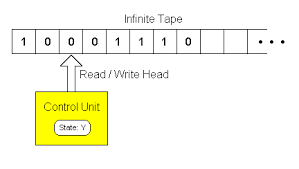
\includegraphics{../images/turingmachine.png}

\textcolor{gray}{"non-deterministic turing machine": itinerary can be represented by a tree...}

\vspace{5mm}


{\fontsize{12pt}{22pt} \textbf{Neural network}\par}

\vspace{5mm}

\underline{Logistic regression with a neural network mindset}

Based on the example from coursera (\textit{deeplearning.ai})

Let us take the example of an image that we want to classify in a \textbf{binary} way: man/woman

The picture is vectorized as a vector of pixels : $\begin{pmatrix}x_1\\...\\x_p\end{pmatrix}$

We use a regression to predict if it's a man/woman:

$y=\omega^Tx + b$

Note: $x$ are all the pixels of \textbf{one} image.

\vspace{5mm}

We want a probability in output (if it's $\ge 0.5$ then we say it's a man).

We thus want the output to be $\widehat{y}=\sigma(\omega^Tx + b)=\mathbb{P}(y|x) \in [0,1]$

(see regression part to get more details on the sigmoid)

\vspace{5mm}

Now since it's a binary classification, we want the $y$ (real value) to be $0$ or $1$.

Thus, the loss function is:

$$\mathcal{L}(y, \widehat{y})=-y\log(\widehat{y})+(1-y)\log(1-\widehat{y})$$

\vspace{5mm}

The cost function is the empiric loss on all examples:

$$J(\omega, b)=\frac{1}{m}\Sigma_{i=1}^m\mathcal{L}(\widehat{y}^{(i)}, y^i)$$

\vspace{5mm}

\underline{Forward propagation}

$$x_1,x_2, \omega_1,\omega_p,b \to z=\omega_1x_1 + \omega_2x_2 + b \to \widehat{y}=a=\sigma(z) \to \mathcal{L}(a,y)$$

- First arrow: regression

- Second arrow: probability

- Third arrow: error

\vspace{5mm}

\underline{Backward propagation}

The idea is: with the error computed on the last step, we go backward in order to correct the parameters $\omega$ and $b$.

$$x_1,x_2, \omega_1,\omega_p,b \leftarrow z=\omega_1x_1 + \omega_2x_2 + b \leftarrow \widehat{y}=a=\sigma(z) \leftarrow \mathcal{L}(a,y)$$

Example: we want to find $\omega_1$ that minimizes the cost function:

$\frac{d\mathcal{L}}{d\omega_1}="d\omega_1"=\frac{d\mathcal{L}}{da}\frac{da}{dz}\frac{dz}{d\omega_1}=...=(a-y)x_1=dzx_1$

Steps:

We compute all the derivatives, then we apply the gradient descent

\lstset{language=Python}
\lstset{frame=lines}
\lstset{caption={Gradient descent (logistic regression with a NN mindset)}}
\lstset{label={lst:code_direct}}
\lstset{basicstyle=\footnotesize}
\begin{lstlisting}

for i in range(num_iterations):
        
     # Cost and gradient calculation
     grads, cost = propagate(w, b, X_train, Y_train) # propagation on ALL the training sample
        
     # Retrieve derivatives from grads
     dw = grads["dw"]
     db = grads["db"]
        
     # update parameters
     w = w - learning_rate * dw
     b = b - learning_rate * db
        
     # Record the costs
     costs.append(cost)

\end{lstlisting}

\lstset{language=Python}
\lstset{frame=lines}
\lstset{caption={Propagation (logistic regression with a NN mindset)}}
\lstset{label={lst:code_direct}}
\lstset{basicstyle=\footnotesize}
\begin{lstlisting}
def propagate(w, b, X, Y):
    
    m = X.shape[1]
    
    # FORWARD PROPAGATION (FROM X TO COST)
    A = sigmoid(np.dot(w.T,X)+b)
    cost = (- 1 / m) * np.sum(Y * np.log(A) + (1 - Y) * (np.log(1 - A))
    
    # BACKWARD PROPAGATION (TO FIND GRAD)
    dw = (1/m)*np.dot(X,(A-Y).T)
    db = (1/m)*np.sum(A-Y)

\end{lstlisting}



\vspace{5mm}
\end{document} 
